\documentclass{beamer}

\usetheme{Madrid}
\usecolortheme{dolphin}

\usepackage[utf8]{inputenc}
\usepackage{hyperref}
\usepackage{graphicx}
\usepackage{amsmath}

\title[Dschungelcamp Simulation]{Dschungelcamp: Agent Simulation of Social Dynamics}
\subtitle{Trust, Reputation, and Alliance Formation in a Reality TV Setting}
\author{LAMY Léo, MUSIL Jan, BUCHKREMER Jan}
\institute[UPM]{Graph Analysis and Social Networks (2025-26)}
\date{\today}

\begin{document}

\begin{frame}
    \titlepage
\end{frame}

\begin{frame}{Table of Contents}
    \tableofcontents
\end{frame}

% ---------------------------------------------------------------
\section{Introduction}
% ---------------------------------------------------------------

\begin{frame}{1. Introduction}
    \begin{itemize}
        \item \textbf{Motivation:} Reality TV shows such as \textit{Ich bin ein Star -- Holt mich hier raus!} (Dschungelcamp) provide a natural laboratory for social dynamics.
        \item \textbf{Setup:} A fixed group of contestants cooperates and competes; periodic votes eliminate one member until only the winner remains.
        \item \textbf{Research Question:} Can we model and reproduce the emergent social structures of such shows using Multi-Agent Systems?
    \end{itemize}
\end{frame}

% ---------------------------------------------------------------
\section{Model Design}
% ---------------------------------------------------------------

\begin{frame}{2. Agent Architecture (BDI)}
    \begin{itemize}
        \item \textbf{Beliefs:} Trust values directed toward each neighbor, perception of own reputation, and current energy levels \cite{Mui}.
        \item \textbf{Desires:} Survive (avoid elimination), maintain energy, and ultimately win (be the last one standing) \cite{Wooldridge}.
        \item \textbf{Intentions:} Strategy-dependent action selection. This includes deciding whether to cooperate or defect during challenges and social encounters, and choosing a specific target during elimination voting \cite{Wooldridge}.
        \item \textbf{Course Parallel:} Maps to Wooldridge's BDI framework for rational agents \cite{Wooldridge}.
    \end{itemize}
\end{frame}

\begin{frame}{3. Agent Strategies \& Personality}
    \begin{columns}[T]
        \begin{column}{0.48\textwidth}
            \textbf{Agent Strategies:}
            \begin{itemize}
                \item \textbf{Cooperator (Green):} Reliable, almost always does challenges to build trust.
                \item \textbf{Strategist (Blue):} Selective cooperation based on current energy and reputation needs.
                \item \textbf{Free-rider (Red):} Avoids challenges, exploiting group resources.
                \item \textbf{Social (Yellow):} Builds connections, highly cooperative in social settings.
            \end{itemize}
        \end{column}
        \begin{column}{0.48\textwidth}
            \textbf{Personality Traits (0.0 - 1.0):}
            \begin{itemize}
                \item \textbf{Openness:} Likelihood to form new social connections. Highest in Social agents (0.8+).
                \item \textbf{Loyalty:} Weight given to existing trust. Highest in Cooperators (0.7+).
                \item \textbf{Bravery:} Willingness to accept energy-draining challenges. Lowest in Free-riders (0.1+).
            \end{itemize}
        \end{column}
    \end{columns}
\end{frame}

\begin{frame}{4. Trust Model (Mui et al.)}
    \begin{itemize}
        \item \textbf{Computational Model:} Direct trust is calculated using a Beta distribution model \cite{Mui}.
        \item \textbf{Formula:} $$T_{ab} = \frac{\alpha + p}{\alpha + \beta + n}$$
        \item \textbf{Parameters:}
        \begin{itemize}
            \item $\alpha, \beta$: Prior parameters (set to 1, 1 for a uniform prior) \cite{Mui}.
            \item $p$: Number of cooperative encounters by agent $B$ observed by $A$.
            \item $n$: Total encounters where $A$ observed $B$'s behavior.
        \end{itemize}
        \item \textbf{Dynamics:} Trust updates after every challenge observation and pairwise social encounter.
    \end{itemize}
\end{frame}

\begin{frame}{5. Gossip \& Reputation}
    \begin{itemize}
        \item \textbf{Gossip (Indirect Trust):} Agents ask a neighbor about a third party, propagating trust indirectly \cite{Mui}.
        \begin{itemize}
            \item Influenced by a \textit{Gossip Spread Factor} ($\gamma = 0.3$).
        \end{itemize}
        \item \textbf{Reputation (Global Score):}
        \begin{itemize}
            \item Calculated as the average of all other active agents' trust IN the target agent \cite{Mui}.
            \item $$R_i = \frac{1}{|N|} \sum_{j \in N} T_{ji}$$
            \item \textbf{Starvation Penalty:} Agents with critically low energy ($< 20$) suffer a $0.1$ reputation penalty, simulating perceived weakness.
        \end{itemize}
    \end{itemize}
\end{frame}

% ---------------------------------------------------------------
\section{Simulation Mechanics}
% ---------------------------------------------------------------

\begin{frame}{6. Simulation Phases \& Elimination}
    Every tick represents one day, split into 4 phases:
    \begin{enumerate}
        \item \textbf{Challenge Phase:} One agent faces a ``Dschungelpr\"{u}fung''. Cooperating earns food but costs energy (-10); defecting saves energy (-3).
        \item \textbf{Food Sharing:} Food pool is distributed to restore energy; daily base energy costs are applied.
        \item \textbf{Social Phase:} Pairwise interactions update direct trust, followed by gossip and alliance updates \cite{Mui}.
        \item \textbf{Elimination:} Every $N$ days, agents vote. The agent with the most votes is eliminated.
    \end{enumerate}
    \vspace{0.2cm}
    \textbf{Voting Logic:} Cooperators punish defectors, Strategists target threats, Free-riders vote defensively, and Socials vote with their alliance \cite{Wooldridge}.
\end{frame}

\begin{frame}{7. Cooperation vs.\ Defection}
    \begin{itemize}
        \item \textbf{Game-Theoretic Framing:} The model presents continuous Prisoner's Dilemma scenarios.
        \item \textbf{Challenges:} Individual vs. Group benefit. Cooperating earns a reward for the shared food pool but drains the individual's energy, making them vulnerable. Defecting preserves individual energy but starves the camp.
        \item \textbf{Social Encounters:} Agents independently decide to cooperate or defect based on their strategy and current trust levels, heavily impacting bidirectional trust updates \cite{Mui}.
    \end{itemize}
\end{frame}

% ---------------------------------------------------------------
\section{Network Analysis \& Results}
% ---------------------------------------------------------------

\begin{frame}{8. Network Structure \& Evolution}
    \begin{itemize}
        \item \textbf{Initialization:} Begins as a complete directed graph where everyone knows everyone (neutral trust = 0.5).
        \item \textbf{Link States \& Visuals:}
        \begin{itemize}
            \item \textbf{Alliance (Green, thick):} Trust $> 0.7$. Prompts formal alliance grouping.
            \item \textbf{Rival (Red, thin):} Trust $< 0.3$.
            \item \textbf{Broken (Hidden):} Trust drops below the $0.2$ threshold.
        \end{itemize}
        \item \textbf{Evolution:} The network shrinks dynamically. When an agent is eliminated, they are moved aside and their directed links are hidden, heavily altering network density and clustering coefficients.
    \end{itemize}
\end{frame}

\begin{frame}{9. Results -- Strategy Survival \& Trust}
    \textbf{Experiment A -- Baseline} (12 agents, 30/30/20 split, gossip on):
    \begin{itemize}
        \item \textbf{Strategy Survival:} Free-riders are eliminated first (all gone by day 12), followed by strategists (day 15) and social agents. Cooperators persist the longest, forming the final survivors.
        \item \textbf{Trust Evolution:} Average trust rises steadily from $0.50 \to 0.95$ over the 33-day season. The steepest increases occur after free-rider eliminations remove the least cooperative agents from the network.
        \item \textbf{Cooperation Rate:} Climbs from $57\%$ to $74\%$ as chronic defectors are voted out, creating a positive feedback loop between cooperation and trust.
    \end{itemize}
\end{frame}

\begin{frame}{10. Results -- Network Metrics \& Cooperation}
    \textbf{Experiment B -- Free-Rider Crash} (80\% free-riders):
    \begin{itemize}
        \item \textbf{Network Density:} Drops from $1.0$ to $0.83$ within just 9 days as widespread defection erodes trust below the link-break threshold ($0.2$). In contrast, the baseline maintains density $\approx 1.0$ throughout.
        \item \textbf{Trust Collapse:} Average trust \emph{falls} from $0.50$ to $0.41$ (vs.\ baseline's rise to $0.95$), and reputation drops to $0.37$.
        \item \textbf{Resource Starvation:} Cooperation rate is only $\sim 32\%$ (vs.\ $74\%$ baseline). Average energy plummets from $90$ to $45$ in 9 days, triggering the starvation penalty ($-0.1$ reputation) across nearly all agents.
    \end{itemize}
\end{frame}

\begin{frame}{11. Demo / NetLogo Interface}
    \begin{center}
        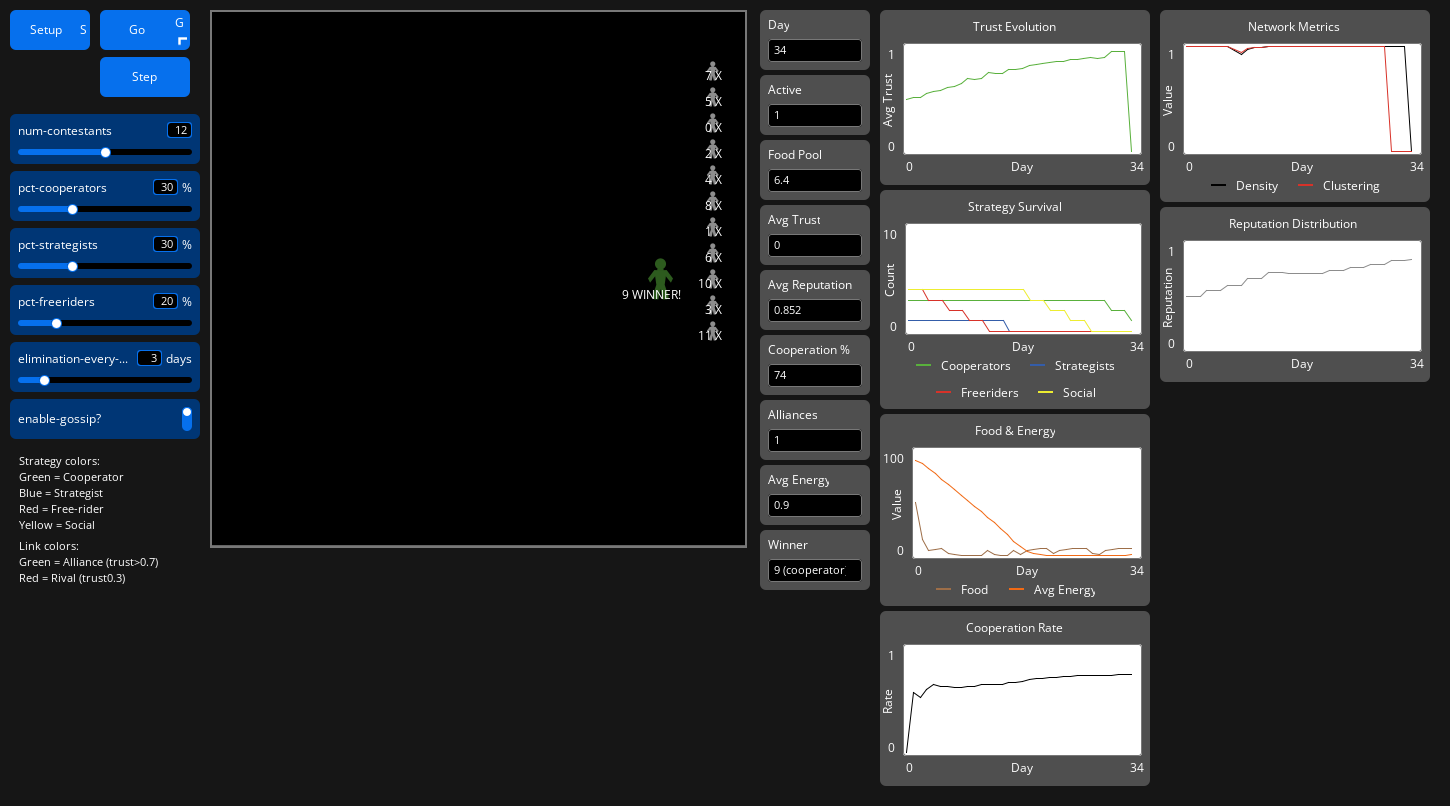
\includegraphics[width=0.9\linewidth]{experiments/baseline/dschungelcamp_interface.png}
    \end{center}
\end{frame}

% ---------------------------------------------------------------
\section{Conclusion}
% ---------------------------------------------------------------

\begin{frame}{12. Conclusion \& Future Work}
    \begin{enumerate}
        \item \textbf{Summary:} The simulation successfully models complex social dynamics, showing how macro-behaviors (alliances, scapegoating) emerge from simple BDI micro-rules and computational trust \cite{Wooldridge, Mui, Hassas}.
        \item \textbf{Key Findings (Experiment C -- 5 runs):} Cooperators are the statistically dominant strategy, winning 4 out of 5 runs (80\%). Their high bravery builds trust capital through consistent challenge participation, which translates into voting protection. Free-riders are eliminated earliest in every run (by day 12) due to chronic defection collapsing their trust scores. Strategists won 1 of 5 runs, surviving through selective cooperation when cooperator numbers were low.
        \item \textbf{Future Work:}
        \begin{itemize}
            \item Integrate \textbf{viewer voting} to simulate external elimination pressure.
            \item Implement dynamic \textbf{challenge difficulty}.
            \item Add \textbf{personality evolution} (agents learning/adapting strategies) and \textbf{resource hoarding}.
        \end{itemize}
    \end{enumerate}
\end{frame}

\begin{frame}{References}
    \footnotesize
    \begin{thebibliography}{99}
        \bibitem{Mui} Mui, L., Mohtashemi, M., \& Halberstadt, A. (2001). \textit{A Computational Model of Trust and Reputation}.
        \bibitem{Wooldridge} Wooldridge, M. (2002). \textit{An Introduction to Multiagent Systems}.
        \bibitem{Hassas} Hassas S., Di Marzo-Serugendo G., Karageorgos A. and Castelfranchi C. (2006). \textit{On self-organising mechanisms}.
    \end{thebibliography}
\end{frame}

\end{document}